\clearpage

\section{Updated predictions of single $\mu$-like ring spectrum in Super-K}
\label{sec:pred}

For 2-flavour oscillations, the predicted reconstructed single $\mu$-like ring spectrum in Super-K depends only on 
$\sin^{2}(2 \theta_{23})$ and $|\Delta m_{32}^{2}|$. However for the 3-flavour hypothesis, it also depends on 
$\sin^{2}(2 \theta_{13})$, $\sin^{2}(2 \theta_{12})$, $\Delta m_{21}^{2}$, $\delta_{CP}$ and the mass hierarchy. 
One other change from the 2-flavour analysis is that oscillated $\nu_{e}$ templates were added for the interaction modes CCQE, CC1$\pi$ and 
CC other. An oscillated $\nu_{e}$ template for NC was not included since the $\nu_{\mu}$ NC template effectively includes $\nu_{e}$ and 
$\nu_{\tau}$ NC.
 
The predicted numbers of events in Super-K for each interaction mode are given in table \ref{genieeventnumbers} for GENIE and in table 
\ref{neuteventnumbers} for NEUT. The 2-flavour predictions are made using $\sin^{2}(2 \theta_{23})$ = 1.0 and $|\Delta m_{32}^{2}|$ = 2.32 $\times$ 10$^{-3}$ eV$^{2}$/c$^{4}$. 
The nominal 3-flavour predictions are made with $\sin^{2}(2 \theta_{12})$ = 0.87, $\sin^{2}(2 \theta_{13})$ = 0.1, $\sin^{2}(2 \theta_{23})$ = 1.0,
$\Delta m_{21}^{2}$ = 7.6 $\times$ 10$^{-5}$ eV$^{2}$/c$^{4}$, $\delta_{CP}$ = 0 and Earth crust density = 2.6 g/cm$^{3}$; the second mass-squared difference 
is 2.32 $\times$ 10$^{-3}$ eV$^{2}$/c$^{4}$ and this is input either as $|\Delta m_{32}^{2}|$ or as $|\Delta m_{FL}^{2}|$ = $|m_{3}^{2} - [(m_{2}^{2} + m_{1}^{2}) / 2]|$. 
The ranges of 3-flavour predictions in tables \ref{genieeventnumbers} and \ref{neuteventnumbers} represent the maximum and minimum numbers from 1000 random 
variations of the non-23 parameters within their uncertainties using the same values of $\sin^{2}(2 \theta_{23})$ and the atmospheric mass-squared difference. 
When the the atmospheric $\Delta m^{2}$ is input as $|\Delta m_{32}^{2}|$, there are more $\nu_{\mu}$ CCQE and 
$\nu_{\mu}$ CC1$\pi$ events in the 3-flavour inverted-hierarchy (IH) prediction and less in the 3-flavour normal-hierarchy (NH) prediction than in the 
2-flavour prediction. This is because the $\nu_{\mu}$-survival probability is higher for the IH than the NH above the oscillation maximum and lower below 
the oscillation maximum (see figure \ref{pnumunumucomp}). Since there are more events above the oscillation maximum than below it, the total number is 
larger for the IH than for the NH. This is true for any combination of the non-23 oscillation parameters. When the the atmospheric $\Delta m^{2}$ is 
input as $|\Delta m_{FL}^{2}|$, the 3-flavour predicted numbers of events are very similar to the 2-flavour numbers; this is because $|\Delta m_{31}^{2}|$ 
is equal to $|\Delta m_{32}^{2}|$ in the 2-flavour approximation, and $|\Delta m_{FL}^{2}|$ represents the average of these two mass-squared differences.


\begin{table}
\caption[Predicted numbers of single $\mu$-like ring events in Super-K for each interaction mode using GENIE]
{Predicted numbers of single $\mu$-like ring events in Super-K for each interaction mode using GENIE. The 2-flavour predictions are made using 
$\sin^{2}(2 \theta_{23})$ = 1.0 and $|\Delta m_{32}^{2}|$ = 2.32 $\times$ 10$^{-3}$ eV$^{2}$/c$^{4}$. The nominal 3-flavour predictions are made with 
$\sin^{2}(2 \theta_{12})$ = 0.87, $\sin^{2}(2 \theta_{13})$ = 0.1, $\sin^{2}(2 \theta_{23})$ = 1.0, $\Delta m_{21}^{2}$ = 7.6 $\times$ 10$^{-5}$ eV$^{2}$/c$^{4}$, 
$\delta_{CP}$ = 0 and Earth crust density = 2.6 g/cm$^{3}$; the second mass-squared difference is 2.32 $\times$ 10$^{-3}$ eV$^{2}$/c$^{4}$ and this is input either 
as $|\Delta m_{32}^{2}|$ or as $|\Delta m_{FL}^{2}|$ = $|m_{3}^{2} - [(m_{2}^{2} + m_{1}^{2}) / 2]|$. The ranges of 3-flavour predictions represent the 
maximum and minimum numbers from 1000 random variations of the non-23 parameters within their uncertainties using the same values of $\sin^{2}(2 \theta_{23})$ 
and the atmospheric mass-squared difference. NH = normal mass hierarchy, IH = inverted mass hierarchy.}
\renewcommand{\tabcolsep}{3.5pt}
\centering
\begin{tabular}{| c | c | c | c | c | c | c | c | c | c |}
\hline
Interaction &  2-flavour & \multicolumn{2}{|c|}{3-flavour} & \multicolumn{2}{|c|}{3-flavour} & \multicolumn{2}{|c|}{3-flavour} & \multicolumn{2}{|c|}{3-flavour} \\
mode &  & \multicolumn{2}{|c|}{$|\Delta m_{32}^{2}|$} & \multicolumn{2}{|c|}{$|\Delta m_{32}^{2}|$} & \multicolumn{2}{|c|}{$|\Delta m_{FL}^{2}|$} & \multicolumn{2}{|c|}{$|\Delta m_{FL}^{2}|$} \\
 &  & \multicolumn{2}{|c|}{(matter, NH)} & \multicolumn{2}{|c|}{(matter, IH)} & \multicolumn{2}{|c|}{(matter, NH)} & \multicolumn{2}{|c|}{(matter, IH)} \\
\hline
 &   & Nominal & Range & Nominal & Range & Nominal & Range & Nominal & Range \\
\hline
Total &  28.39 & 28.14 & 28.06 & 28.87 & 28.56 & 28.51 & 28.44 & 28.45 & 28.17 \\
 &  &  & - 28.43  &  & - 28.98 &  & - 28.83 &  & - 28.52 \\
\hline
$\nu_{\mu}$ CCQE &  16.52 & 16.32 & 16.27 & 16.79 & 16.59 & 16.55 & 16.50 & 16.51 & 16.33 \\
 &  (58.1\%) & (58.0\%) & - 16.49 & (58.2\%) & - 16.87 & (58.0\%) & - 16.76 & (58.0\%) & - 16.55 \\
\hline
$\nu_{\mu}$ CC1$\pi$ &  6.68 & 6.56 & 6.55 & 6.78 & 6.70 & 6.68 & 6.66 & 6.66 & 6.58 \\
 &  (23.6\%) &(23.3\%) & - 6.64  &(23.5\%) & - 6.81 & (23.4\%) & 6.76 & (23.4\%) & - 6.68 \\
\hline
$\nu_{\mu}$ CCother &  1.11 & 1.10 & 1.10 & 1.11 & 1.11 & 1.11 & 1.11 & 1.11 & 1.10 \\
 & (3.9\%)  & (3.4\%) & - 1.10 & (3.8\%) & - 1.11 & (3.9\%) & - 1.11 & (3.9\%) & - 1.11\\
\hline
$\nu_{\mu}$ ($\nu_{\tau}$) NC &  2.12 & 2.12 & 2.12 & 2.12 & 2.12 & 2.12 & 2.12 & 2.12 & 2.12 \\
 &  (7.5\%) & (7.5\%) & - 2.12 & (7.3\%) & -2.12 & (7.4\%) & - 2.12 & (7.4\%) & - 2.12 \\
\hline
$\bar{\nu}_{\mu}$ CCQE &  1.05 & 1.05 & 1.05 & 1.07 & 1.07 & 1.07 & 1.06 & 1.06 & 1.05 \\
 &  (3.7\%) & (3.7\%) & - 1.05 & (3.7\%) & -1.08 & (3.7\%) & - 1.07 & (3.7\%) & - 1.06 \\
\hline
$\bar{\nu}_{\mu}$ CC1$\pi$ &  0.63 & 0.64 & 0.64 & 0.65 & 0.65 & 0.64 & 0.64 & 0.64 & 0.64 \\
 &  (2.3\%) & (2.3\%) & - 0.64 & (2.3\%) & - 0.65 & (2.3\%) & - 0.65 & (2.3\%) & - 0.64 \\
\hline
$\bar{\nu}_{\mu}$ CCother &  0.11 & 0.11 & 0.11 & 0.11 & 0.11 & 0.11 & 0.11 & 0.11 & 0.11 \\
 &  (0.4\%) & (0.4\%) & - 0.11 & (0.4\%) & - 0.11 & (0.4\%) & - 0.11 & (0.4\%) & - 0.11 \\
\hline
$\bar{\nu}_{\mu}$ ($\bar{\nu}_{\tau}$) NC &  0.12 & 0.12 & 0.12 & 0.12 & 0.12 & 0.12 & 0.12 & 0.12 & 0.12 \\
 &  (0.4\%) & (0.4\%) & - 0.12 & (0.4\%) & - 0.12 & (0.4\%) & - 0.12 & (0.4\%) & - 0.12 \\
\hline
$\nu_{e}$ CCQE &  0.007 & 0.006 & 0.006 & 0.007 & 0.006 & 0.006 & 0.006 & 0.007 & 0.006 \\
(background) & (0.02\%) & (0.02\%) & - 0.007 & (0.02\%) & - 0.007 & (0.02\%) & - 0.007 & (0.02\%) & - 0.007 \\
\hline
$\nu_{e}$ CC1$\pi$ &  0.004 & 0.004 & 0.004 & 0.004 & 0.004 & 0.004 & 0.004 & 0.004 & 0.004 \\
(background) & (0.01\%) & (0.01\%) & - 0.004 & (0.01\%) & - 0.004 & (0.01\%) & - 0.004 & (0.01\%) & - 0.004 \\
\hline
$\nu_{e}$ CCother &  0.001 & 0.001 & 0.001 & 0.001 & 0.001 & 0.001 & 0.001 & 0.001 & 0.001 \\
(background) & (0.003\%) & (0.003\%) & - 0.001 & (0.003\%) & - 0.001 & (0.003\%) & - 0.001 & (0.003\%) & - 0.001 \\
\hline
$\nu_{e}$ NC & 0.06 & 0.06 & 0.06 & 0.06 & 0.06 & 0.06 & 0.06 & 0.06 & 0.06 \\
(background) & (0.2\%) & (0.2\%) & - 0.06  & (0.2\%) & - 0.06 & (0.2\%) & - 0.06 & (0.2\%) & - 0.06 \\
\hline
$\nu_{e}$ CCQE &  & 0.04 & 0.02 & 0.04 & 0.02  & 0.04 & 0.02 & 0.04 & 0.01 \\
(oscillated) &  & (0.1\%) & - 0.07 & (0.1\%) & - 0.06 & (0.1\%) & - 0.07 & (0.1\%) & - 0.06 \\
\hline
$\nu_{e}$ CC1$\pi$ &  & 0.01 & 0.004 & 0.01 & 0.004 & 0.01 & 0.005 & 0.01 & 0.005 \\
(oscillated) &  & (0.04\%) & - 0.02 & (0.03\%)  & - 0.017 & (0.05\%) & - 0.02 & (0.04\%) & - 0.017 \\
\hline
$\nu_{e}$ CCother &  & 0.0006 & 0.0002 & 0.0004 & 0.0002 & 0.0006 & 0.0002 & 0.0004 & 0.0002 \\
(oscillated) &  & (0.002\%) & - 0.0008 & (0.001\%) & - 0.0007 & (0.002\%) & - 0.0009 & (0.001\%) & - 0.0007 \\
\hline
\end{tabular}
\label{genieeventnumbers}
\end{table}

\begin{table}
\caption[Predicted numbers of single $\mu$-like ring events in Super-K for each interaction mode using NEUT]
{Predicted numbers of single $\mu$-like ring events in Super-K for each interaction mode using NEUT. The 2-flavour predictions are made using
$\sin^{2}(2 \theta_{23})$ = 1.0 and $|\Delta m_{32}^{2}|$ = 2.32 $\times$ 10$^{-3}$ eV$^{2}$/c$^{4}$. The nominal 3-flavour predictions are made with
$\sin^{2}(2 \theta_{12})$ = 0.87, $\sin^{2}(2 \theta_{13})$ = 0.1, $\sin^{2}(2 \theta_{23})$ = 1.0, $\Delta m_{21}^{2}$ = 7.6 $\times$ 10$^{-5}$ eV$^{2}$/c$^{4}$,
$\delta_{CP}$ = 0 and Earth crust density = 2.6 g/cm$^{3}$; the second mass-squared difference is 2.32 $\times$ 10$^{-3}$ eV$^{2}$/c$^{4}$ and this is input either
as $|\Delta m_{32}^{2}|$ or as $|\Delta m_{FL}^{2}|$ = $|m_{3}^{2} - [(m_{2}^{2} + m_{1}^{2}) / 2]|$. The ranges of 3-flavour predictions represent the
maximum and minimum numbers from 1000 random variations of the non-23 parameters within their uncertainties using the same values of $\sin^{2}(2 \theta_{23})$
and the atmospheric mass-squared difference. NH = normal mass hierarchy, IH = inverted mass hierarchy.}
\renewcommand{\tabcolsep}{3.5pt}
\centering
\begin{tabular}{| c | c | c | c | c | c | c | c | c | c |}
\hline
Interaction &  2-flavour & \multicolumn{2}{|c|}{3-flavour} & \multicolumn{2}{|c|}{3-flavour} & \multicolumn{2}{|c|}{3-flavour} & \multicolumn{2}{|c|}{3-flavour} \\
mode &  & \multicolumn{2}{|c|}{$|\Delta m_{32}^{2}|$} & \multicolumn{2}{|c|}{$|\Delta m_{32}^{2}|$} & \multicolumn{2}{|c|}{$|\Delta m_{FL}^{2}|$} & \multicolumn{2}{|c|}{$|\Delta m_{FL}^{2}|$} \\
 &  & \multicolumn{2}{|c|}{(matter, NH)} & \multicolumn{2}{|c|}{(matter, IH)} & \multicolumn{2}{|c|}{(matter, NH)} & \multicolumn{2}{|c|}{(matter, IH)} \\
\hline
 &   & Nominal & Range & Nominal & Range & Nominal & Range & Nominal & Range \\
\hline
Total & 29.18 & 28.86  & 28.79 &  29.74 & 29.40 & 29.31 & 29.23 & 29.23 & 28.92 \\
 &  &   & - 29.26  &   & - 29.86 & & - 29.70 &  & - 29.33 \\
\hline
$\nu_{\mu}$ CCQE & 16.73 & 16.49 & 16.45 & 17.08 & 16.85 & 16.79 & 16.73 & 16.74 & 16.54 \\
 &(57.3\%) &  (57.1\%) & - 16.75 & (57.5\%) & - 17.17 & (57.3\%) & - 17.05 & (57.3\%) & - 16.80 \\
\hline
$\nu_{\mu}$ CC1$\pi$ & 7.01 &  6.90 & 6.87 & 7.14 & 7.05 & 7.02 & 7.00 & 7.01 & 6.93 \\
 & (24.0\%) & (23.9\%) & - 6.99 & (24.0\%) & - 7.16 & (24.0\%) & - 7.11 & (24.0\%) & - 7.03 \\
\hline
$\nu_{\mu}$ CCother & 1.80 & 1.79  & 1.79 &  1.81 & 1.80 & 1.80 & 1.80 & 1.80 & 1.79 \\
 & (6.2\%) & (6.2\%)  & - 1.80 &  (6.1\%) & - 1.81 &  (6.1\%) & - 1.81 &  (6.2\%) & - 1.80 \\
\hline
$\nu_{\mu}$ ($\nu_{\tau}$) NC & 1.68 & 1.69 & 1.69 & 1.69 & 1.69 & 1.69 & 1.69 & 1.69 & 1.69 \\
 & (5.7\%) & (5.8\%) & - 1.69 &  (5.7\%) & - 1.69 &  (5.8\%) & - 1.69 &  (5.8\%) & - 1.69 \\
\hline
$\bar{\nu}_{\mu}$ CCQE & 1.11 &  1.10 & 1.10 &  1.13 & 1.12 & 1.11 & 1.11 & 1.11 & 1.10 \\
 & (3.8\%) &  (3.8\%) & - 1.11 &  (3.8\%) & - 1.13 &  (3.8\%) & - 1.12 &  (3.8\%) & - 1.11 \\
\hline
$\bar{\nu}_{\mu}$ CC1$\pi$ & 0.51 &  0.51 & 0.50 &  0.51 & 0.51 & 0.51 & 0.51 & 0.51 & 0.51 \\
 & (1.7\%) &  (1.8\%) & - 0.51 &  (1.7\%) & - 0.52 &  (1.7\%) & - 0.51 &  (1.7\%) & 0.51 \\
\hline
$\bar{\nu}_{\mu}$ CCother & 0.17 &  0.17 & 0.17 & 0.17 & 0.17 & 0.17 & 0.17 & 0.17 & 0.17 \\
 & (0.6\%) &  (0.6\%) & - 0.17 &  (0.6\%) & - 0.17 &  (0.6\%) & - 0.17 &  (0.6\%) & - 0.17 \\
\hline
$\bar{\nu}_{\mu}$ ($\bar{\nu}_{\tau}$) NC & 0.093 & 0.093 & 0.093 &  0.093 & 0.093 & 0.093 & 0.093 & 0.093 & 0.093 \\
 & (0.3\%) & (0.3\%) & - 0.093 &  (0.3\%) & - 0.093 &  (0.3\%) & - 0.093 &  (0.3\%) & 0.093 \\
\hline
$\nu_{e}$ CCQE & 0.008 &  0.007 & 0.007 & 0.007 & 0.007 & 0.007 & 0.007 & 0.007 & 0.007 \\
(background) & (0.03\%) &  (0.02\%) & - 0.007 & (0.02\%) & - 0.007 &  (0.02\%) & - 0.007 &  (0.02\%) & - 0.007 \\
\hline
$\nu_{e}$ CC1$\pi$ & 0.005 & 0.004 & 0.004 &  0.004 & 0.004 & 0.004 & 0.004 & 0.004 & 0.004 \\
(background) & (0.02\%) & (0.02\%) & - 0.004 & (0.01\%) & - 0.004 & (0.01\%)  & 0.004 & (0.01\%) & - 0.004 \\
\hline
$\nu_{e}$ CCother & 0.002 &  0.001 & 0.001 & 0.001 & 0.001 & 0.001 & 0.001 & 0.001 & 0.001 \\
(background) & (0.006\%) &  (0.005\%) & - 0.001 &  (0.005\%) & - 0.001 &  (0.005\%) & - 0.001 &  (0.005\%) & - 0.001 \\
\hline
$\nu_{e}$ NC & 0.05 &  0.05 & 0.05 & 0.05 & 0.05 & 0.05 & 0.05 & 0.05 & 0.05 \\
(background) & (0.2\%) &  (0.2\%) & - 0.05 &  (0.2\%) & - 0.05 &  (0.2\%) & - 0.05 &  (0.2\%) & - 0.05 \\
\hline
$\nu_{e}$ CCQE &  &  0.04 & 0.02 & 0.04 & 0.02 & 0.04 & 0.02 & 0.04 & 0.02 \\
(oscillated) &  &  (0.1\%) & - 0.07 & (0.1\%) & - 0.06 & (0.1\%) & - 0.07 & (0.1\%) & - 0.06 \\
\hline
$\nu_{e}$ CC1$\pi$ &   &  0.015 & 0.006 & 0.01 & 0.006& 0.01 & 0.005 & 0.01 & 0.005 \\
(oscillated) &  &  (0.04\%) & - 0.023 & (0.04\%) & - 0.020 & (0.05\%) & - 0.022 & (0.04\%) & - 0.021 \\
\hline
$\nu_{e}$ CCother &  &  0.001 & 0.0007 &  0.001 & 0.0006 & 0.001 & 0.0005 & 0.001 & 0.0005 \\
(oscillated) &  &  (0.005\%) & - 0.0022 &  (0.004\%) & - 0.0019 &  (0.005\%) & - 0.0021 &  (0.004\%) & - 0.0020\\
\hline
\end{tabular}
\label{neuteventnumbers}
\end{table}


The predicted reconstructed single-ring $\mu$-like Super-K spectrum using GENIE is shown in the upper plot of figure \ref{sknominalgenie}. In this plot, 
3-flavour spectra are shown both for the value 2.32 $\times$ 10$^{-3}$ eV$^{2}$/c$^{4}$ input as $|\Delta m_{32}^{2}|$ and for the same value input as 
$|\Delta m_{FL}^{2}|$ for both the NH and IH. The 2-flavour predicted spectrum is also shown for comparison. The lower plot shows the ratios of all four 
3-flavour spectra to the 2-flavour spectrum. The equivalent plots using NEUT are shown in figure \ref{sknominalneut}. These figures also show that, when 
the atmospheric $\Delta m^{2}$ is input as $|\Delta m_{32}^{2}|$, more events are predicted above the oscillation maximum and less below it for the IH 
than for the NH. When the the atmospheric $\Delta m^{2}$ is input as $|\Delta m_{FL}^{2}|$, they show that the 3-flavour predicted spectra are very similar 
to the 2-flavour spectra.

The effects of uncertainties in the non-23 oscillation parameters on the predicted reconstructed single-ring $\mu$-like Super-K spectrum are 
shown in figures \ref{skratiotheta13}, \ref{skratiodeltacp}, \ref{skratiotheta12} and \ref{skratiodm12sq}. For greater clarity, these effects are shown 
as ratios of the spectrum for $\pm$1$\sigma$ variations of a single oscillation parameter to that for the nominal value of that parameter, with the 
other five oscillation parameters being fixed. The uncertainties in $\sin^{2}(2 \theta_{12})$ and $\Delta m_{21}^{2}$ are taken from KamLAND combined 
with solar experiments \cite{Kamland}, while those in $\sin^{2}(2 \theta_{13})$ are computed as a weighted average of measurements from Daya Bay 
\cite{DayaBay} and Reno \cite{Reno}. 

By far the largest effect on the Super-K spectrum is from uncertainties in $\delta_{CP}$: changing this parameter from 0 to $\pi$ results in an 
increase of up to 5\% in the spectrum above the oscillation maximum and a decrease of up to 3\% below it for the NH. These changes 
in the spectrum are due to the changes in P($\nu_{\mu}\rightarrow\nu_{\mu}$) for different values of $\delta_{CP}$ shown in figure \ref{pnumunumudelta} 
and described in section \ref{sec:nuosc3f}. The effect 
of $\delta_{CP}$ on the predicted Super-K spectrum depends on the value of $\theta_{13}$ since the $e^{i\delta}$ terms in the PMNS matrix 
(equation \ref{PMNSmatrix}) are always multiplied by $\sin(\theta_{13})$; in figure \ref{skratiodeltacp}, $\sin^{2}(2 \theta_{13})$ has the value 
0.1. The effects of uncertainties in the other three non-23 parameters are smaller, and in all cases change the predicted Super-K spectrum by 
$\leq$ 0.5\%. For the NH, an increase in the values of both $\sin^{2}(2 \theta_{12})$ and $\Delta m_{21}^{2}$ results in an increase 
in the predicted numbers of events at energies below the oscillation maximum, and a decrease in them above the oscillation maximum; these changes 
are due to the changes in P($\nu_{\mu}\rightarrow\nu_{\mu}$) for different values of $\sin^{2}(2 \theta_{12})$ and $\Delta m_{21}^{2}$ shown in 
table \ref{numuSurvProbEffectError12}. The effects of 
$\delta_{CP}$, $\sin^{2}(2 \theta_{12})$ and $\Delta m_{21}^{2}$ are all reversed for the inverted hierarchy. The effect of an increase in 
$\sin^{2}(2 \theta_{13})$ is to increase the predicted number of events in Super-K for both hierarchies, while a decrease in this parameter results 
in a decrease in the predicted number. This is because an increase in $\sin^{2}(2 \theta_{13})$ increases P($\nu_{\mu}\rightarrow\nu_{\mu}$) for a 
given value of $\sin^{2}(2 \theta_{23})$ as shown in figure \ref{pnumunumus13}, i.e.\ more $\nu_{\mu}$ survive for higher values of $\sin^{2}(2 \theta_{13})$.

\begin{figure}
\begin{center}
\resizebox{14cm}{!}{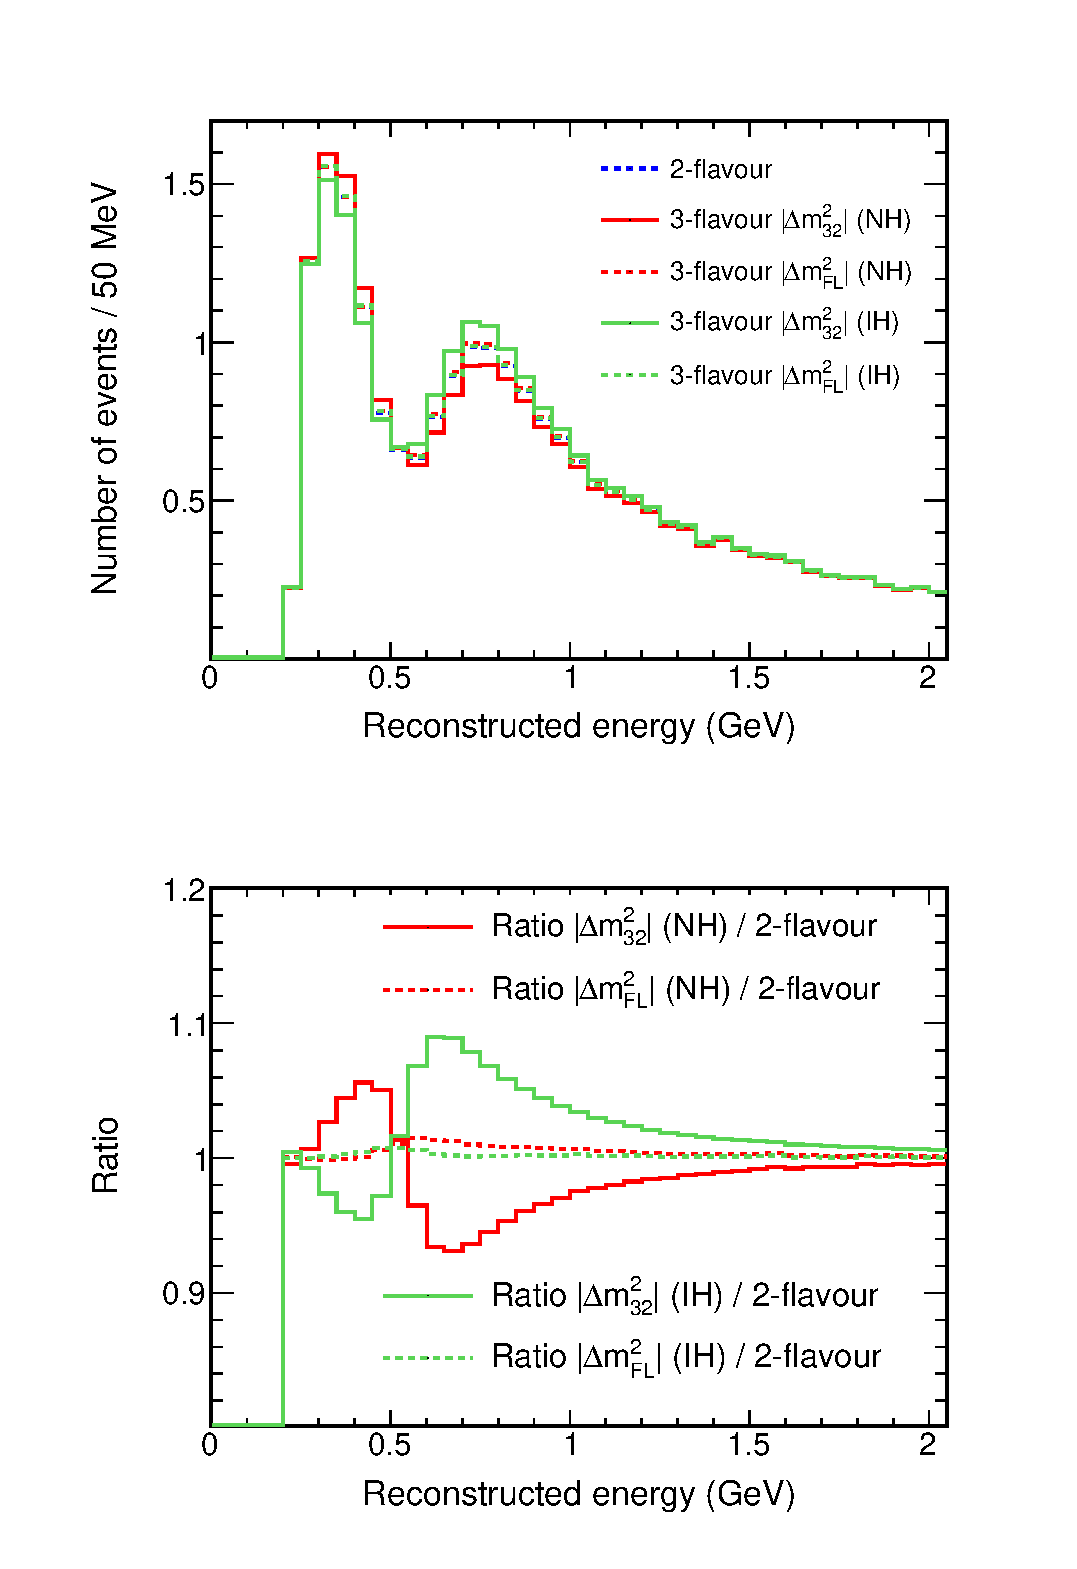
\includegraphics{./images/predicted_spectrum/SKErecoNominalGenie.eps}}
\caption[Predicted reconstructed single $\mu$-like ring spectra in Super-K for the 2-flavour and 3-flavour (in matter) hypotheses using GENIE (top plot) 
and ratios of the 3-flavour spectra to the 2-flavour spectrum (bottom plot)]
{Predicted reconstructed single $\mu$-like ring spectra in Super-K for the 2-flavour and 3-flavour (in matter) hypotheses using GENIE (top); for the 
3-flavour spectra, the value 2.32 $\times$ 10$^{-3}$ eV$^{2}$/c$^{4}$ input either as $|\Delta m_{32}^{2}|$ or as $|\Delta m_{FL}^{2}|$
= $|m_{3}^{2} - [(m_{2}^{2} + m_{1}^{2}) / 2]|$. The ratios of the 3-flavour spectra to the 2-flavour spectrum are shown in the bottom plot;  
$\sin^{2}(2 \theta_{12})$ = 0.87, $\sin^{2}(2 \theta_{13})$ = 0.1, $\sin^{2}(2 \theta_{23})$ = 1.0, $\Delta m_{21}^{2}$ = 7.6 $\times 10^{-5}$ eV$^{2}$/c$^{4}$, 
$\delta_{CP}$ = 0, Earth crust density = 2.6 g/cm$^{3}$, NH = normal mass hierarchy and IH = inverted mass hierarchy.}
\label{sknominalgenie}
\end{center}
\end{figure}

\begin{figure}
\begin{center}
\resizebox{14cm}{!}{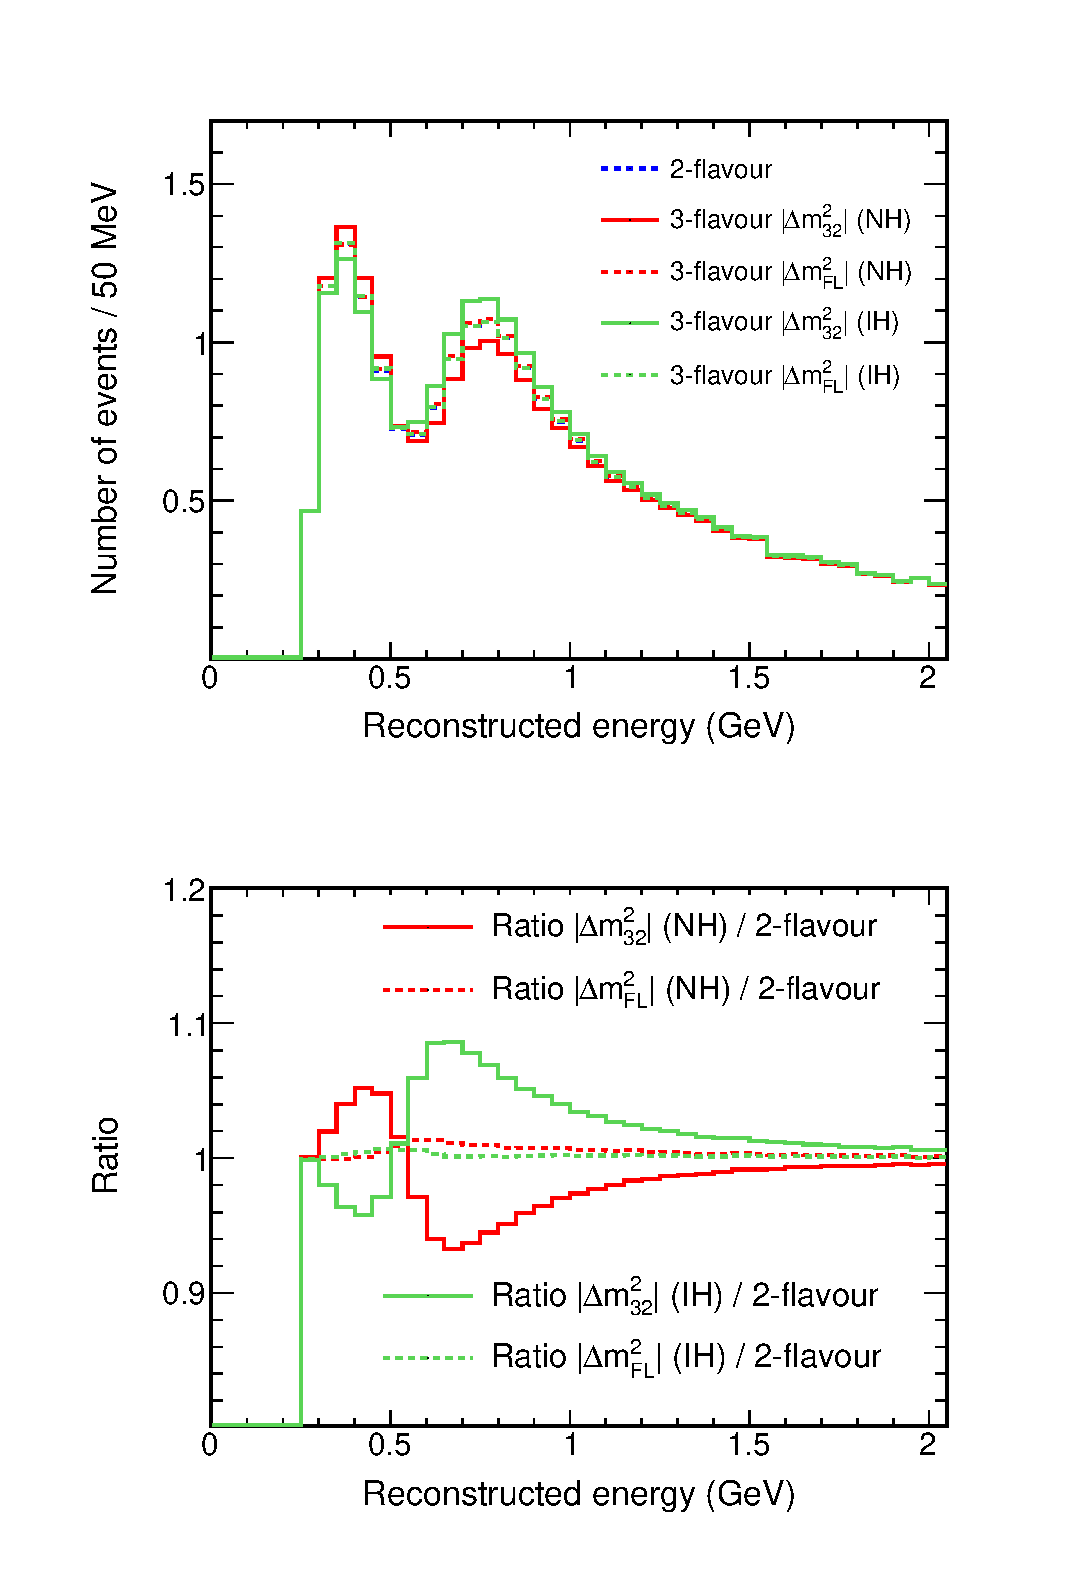
\includegraphics{./images/predicted_spectrum/SKErecoNominalNeut.eps}}
\caption[Predicted reconstructed single $\mu$-like ring spectra in Super-K for the 2-flavour and 3-flavour (in matter) hypotheses using NEUT (top plot)
and ratios of the 3-flavour spectra to the 2-flavour spectrum (bottom plot)]
{Predicted reconstructed single $\mu$-like ring spectra in Super-K for the 2-flavour and 3-flavour (in matter) hypotheses using NEUT (top); for the 
3-flavour spectra, the value 2.32 $\times$ 10$^{-3}$ eV$^{2}$/c$^{4}$ input either as $|\Delta m_{32}^{2}|$ or as $|\Delta m_{FL}^{2}|$
= $|m_{3}^{2} - [(m_{2}^{2} + m_{1}^{2}) / 2]|$. The ratios of the 3-flavour spectra to the 2-flavour spectrum are shown in the bottom plot;
$\sin^{2}(2 \theta_{12})$ = 0.87, $\sin^{2}(2 \theta_{13})$ = 0.1, $\sin^{2}(2 \theta_{23})$ = 1.0, $\Delta m_{21}^{2}$ = 7.6 $\times 10^{-5}$ eV$^{2}$/c$^{4}$,
$\delta_{CP}$ = 0, Earth crust density = 2.6 g/cm$^{3}$, NH = normal mass hierarchy and IH = inverted mass hierarchy.}
\label{sknominalneut}
\end{center}
\end{figure}

\clearpage

\begin{figure}
\begin{center}
\resizebox{13cm}{!}{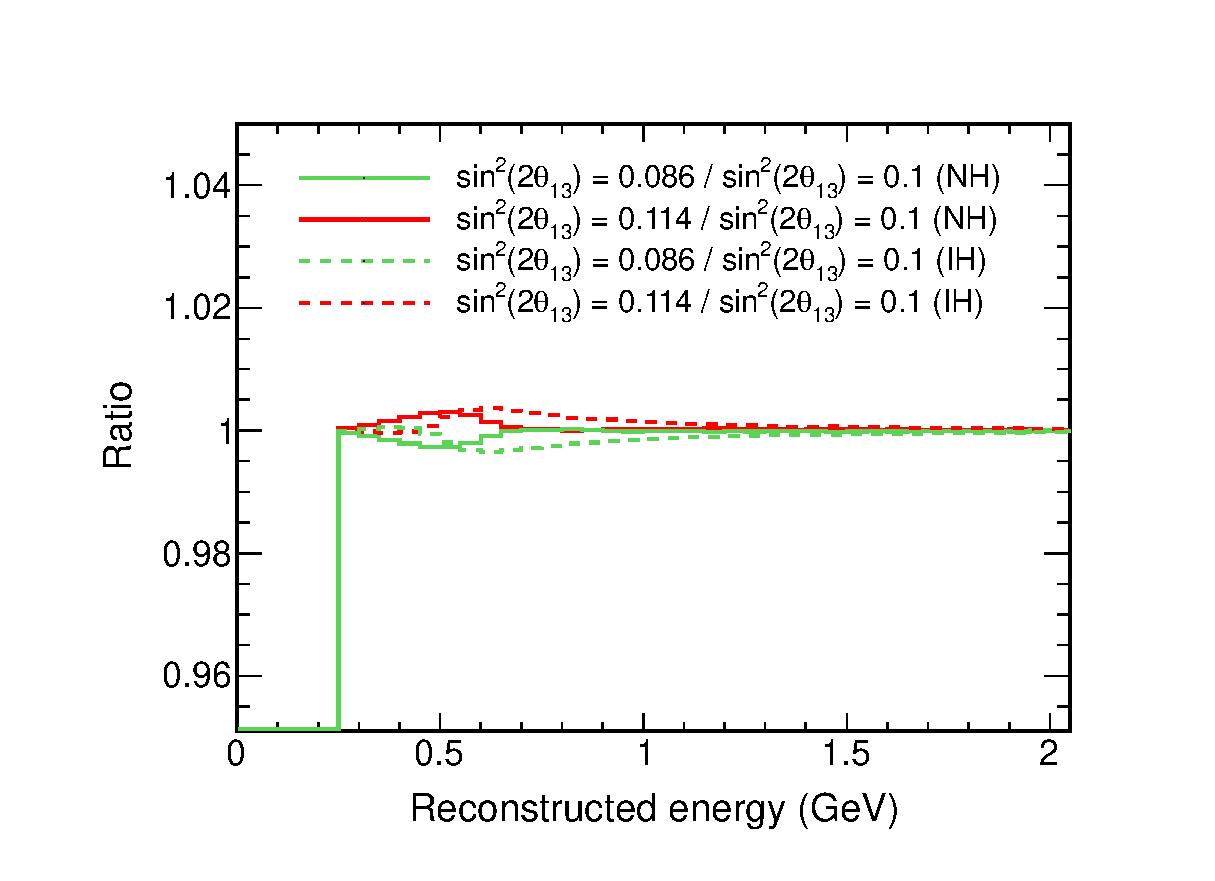
\includegraphics{./images/predicted_spectrum/SKErecoRatioTheta13.eps}}
\caption[Ratios of predicted reconstructed single $\mu$-like ring spectra in Super-K for $\pm$1$\sigma$ variations in
$\sin^{2}(2 \theta_{13})$ to those for the nominal value using NEUT]
{Ratios of predicted reconstructed single $\mu$-like ring spectra in Super-K for $\pm$1$\sigma$ variations in 
$\sin^{2}(2 \theta_{13})$ to those for the nominal value using NEUT; $\sin^{2}(2 \theta_{12})$ = 0.87, $\sin^{2}(2 \theta_{23})$ = 1.0, 
$\Delta m_{21}^{2}$ = 7.6 $\times 10^{-5}$ eV$^{2}$/c$^{4}$, $|\Delta m_{32}^{2}|$ = 2.32 $\times$ 10$^{-3}$ eV$^{2}$/c$^{4}$, $\delta_{CP}$ = 0, 
Earth crust density = 2.6 g/cm$^{3}$, NH = normal mass hierarchy and IH = inverted mass hierarchy}
\label{skratiotheta13}
\end{center}
\end{figure}

\begin{figure}
\begin{center}
\resizebox{13cm}{!}{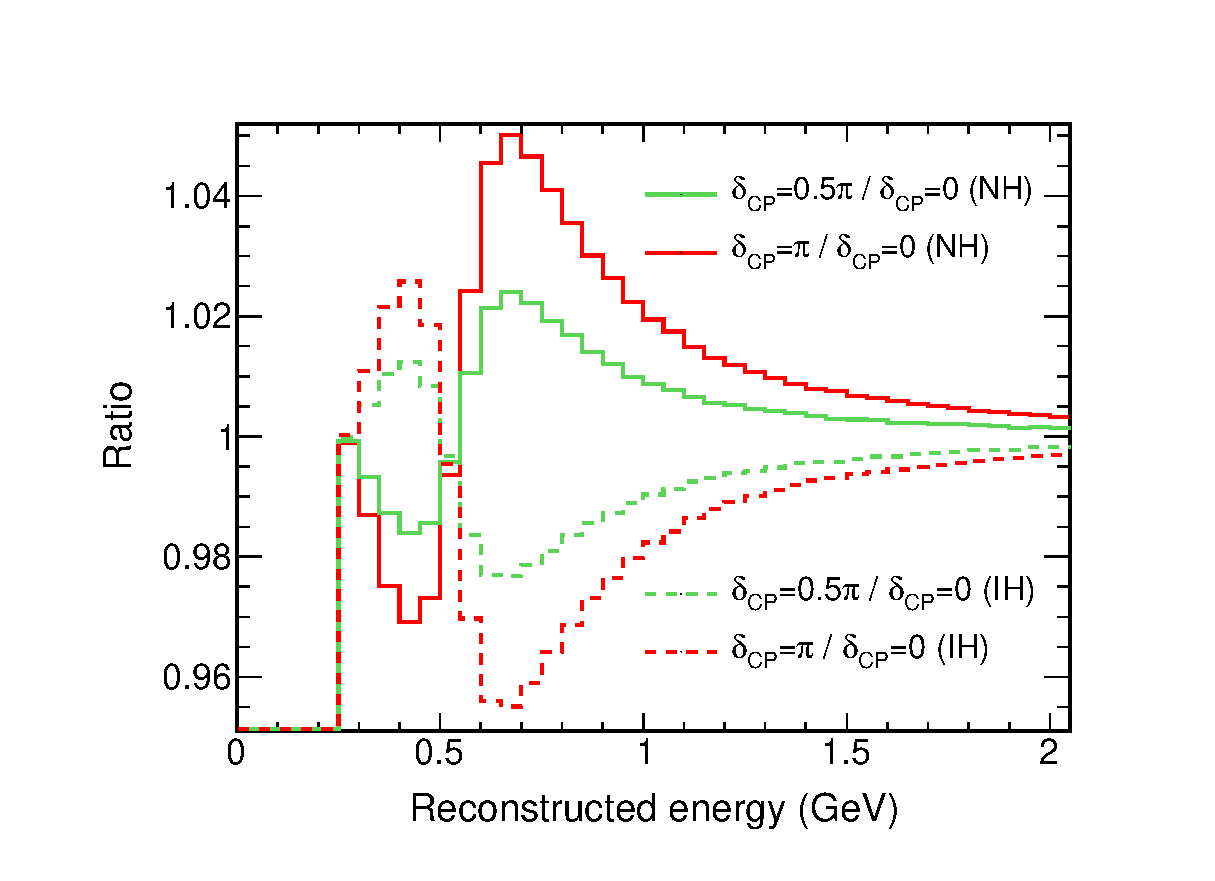
\includegraphics{./images/predicted_spectrum/SKErecoRatioDeltaCP.eps}}
\caption[Ratios of predicted reconstructed single $\mu$-like ring spectra in Super-K for $\delta_{CP}$ = $\pi$/2 and
$\delta_{CP}$ = $\pi$ to those for $\delta_{CP}$ = 0 using NEUT]
{Ratios of predicted reconstructed single $\mu$-like ring spectra in Super-K for $\delta_{CP}$ = $\pi$/2 and 
$\delta_{CP}$ = $\pi$ to those for $\delta_{CP}$ = 0 using NEUT; $\sin^{2}(2 \theta_{12})$ = 0.87, $\sin^{2}(2 \theta_{13})$ = 0.1, 
$\sin^{2}(2 \theta_{23})$ = 1.0, $\Delta m_{21}^{2}$ = 7.6 $\times 10^{-5}$ eV$^{2}$/c$^{4}$,$|\Delta m_{32}^{2}|$ 
= 2.32 $\times$ 10$^{-3}$ eV$^{2}$/c$^{4}$, Earth crust density = 2.6 g/cm$^{3}$, NH = normal mass hierarchy and IH = inverted mass hierarchy}
\label{skratiodeltacp}
\end{center}
\end{figure}

\clearpage

\begin{figure}
\begin{center}
\resizebox{13cm}{!}{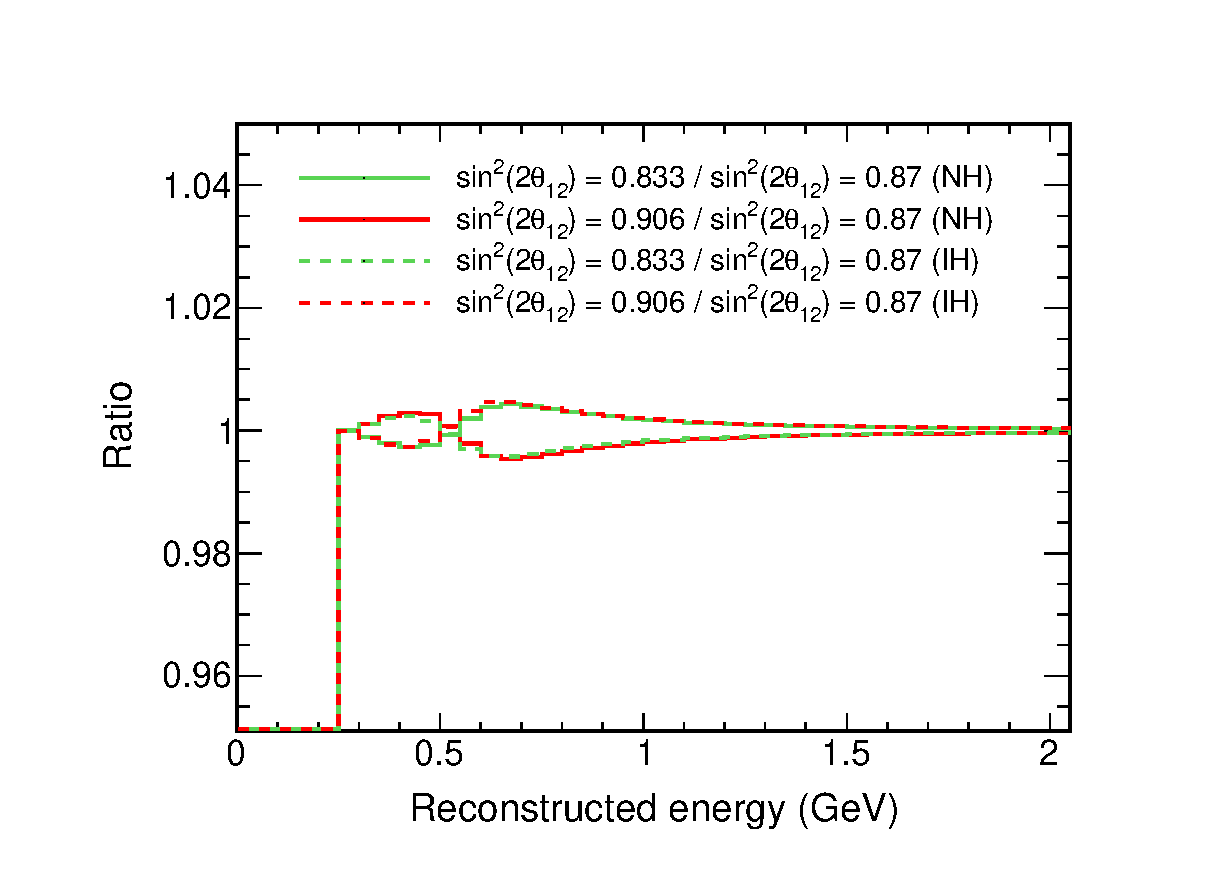
\includegraphics{./images/predicted_spectrum/SKErecoRatioTheta12.eps}}
\caption[Ratios of predicted reconstructed single $\mu$-like ring spectra in Super-K for $\pm$1$\sigma$ variations in
$\sin^{2}(2 \theta_{12})$ to those for the nominal value using NEUT]
{Ratios of predicted reconstructed single $\mu$-like ring spectra in Super-K for $\pm$1$\sigma$ variations in
$\sin^{2}(2 \theta_{12})$ to those for the nominal value using NEUT; $\sin^{2}(2 \theta_{13})$ = 0.1, $\sin^{2}(2 \theta_{23})$ = 1.0,
$\Delta m_{21}^{2}$ = 7.6 $\times 10^{-5}$ eV$^{2}$/c$^{4}$, $|\Delta m_{32}^{2}|$ = 2.32 $\times$ 10$^{-3}$ eV$^{2}$/c$^{4}$, $\delta_{CP}$ = 0, 
Earth crust density = 2.6 g/cm$^{3}$, NH = normal mass hierarchy and IH = inverted mass hierarchy}
\label{skratiotheta12}
\end{center}
\end{figure}

\begin{figure}
\begin{center}
\resizebox{13cm}{!}{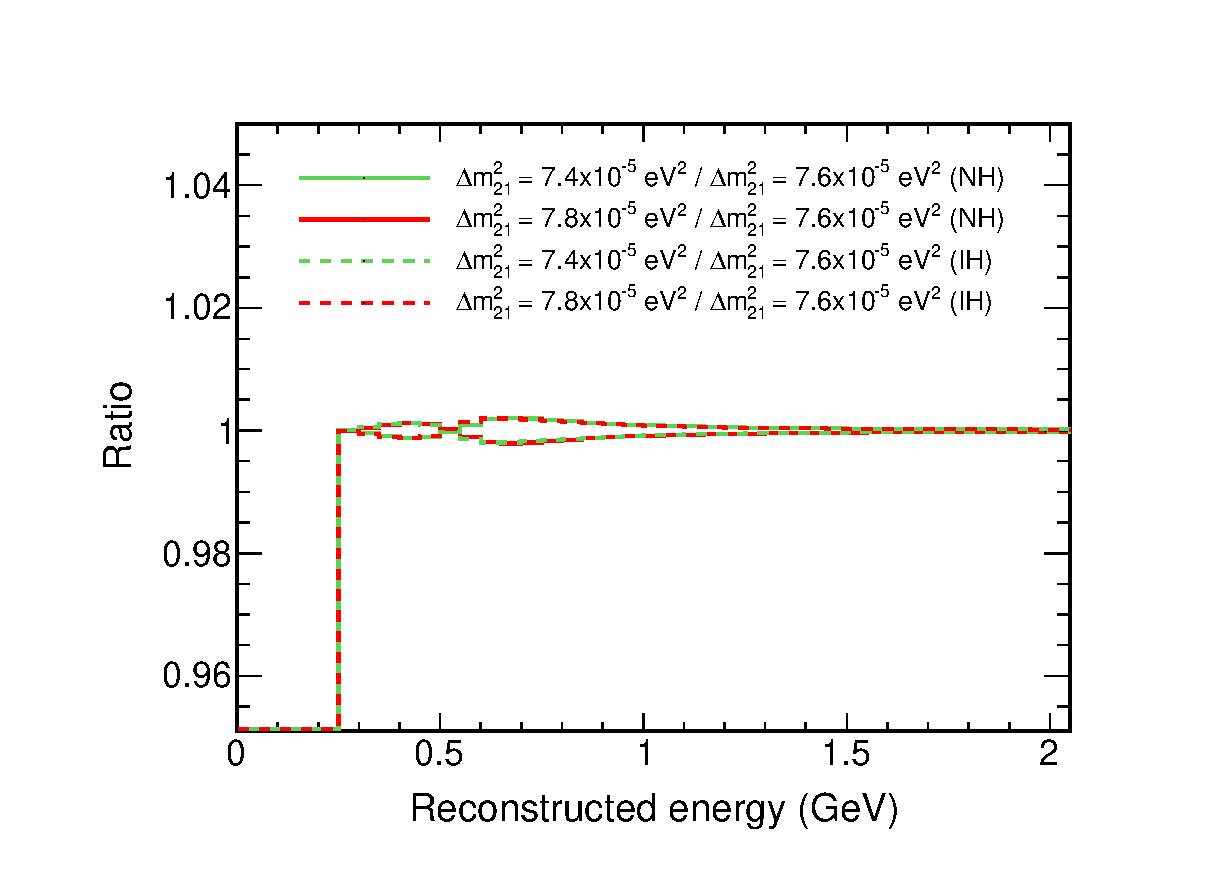
\includegraphics{./images/predicted_spectrum/SKErecoRatioDm12sq.eps}}
\caption[Ratios of predicted reconstructed single $\mu$-like ring spectra in Super-K for $\pm$1$\sigma$ variations in
$\Delta m_{21}^{2}$ to those for the nominal value using NEUT]
{Ratios of predicted reconstructed single $\mu$-like ring spectra in Super-K for $\pm$1$\sigma$ variations in
$\Delta m_{21}^{2}$ to those for the nominal value using NEUT; $\sin^{2}(2 \theta_{12})$ = 0.87, $\sin^{2}(2 \theta_{13})$ = 0.1, 
$\sin^{2}(2 \theta_{23})$ = 1.0, $|\Delta m_{32}^{2}|$ = 2.32 $\times$ 10$^{-3}$ eV$^{2}$/c$^{4}$, $\delta_{CP}$ = 0, Earth 
crust density = 2.6 g/cm$^{3}$, NH = normal mass hierarchy and IH = inverted mass hierarchy}
\label{skratiodm12sq}
\end{center}
\end{figure}

\clearpage











